This part is responsible for doing the interpretation between the two different modules i.e. the Model module and the MCTS Algorithm module, our AI . The Model and the AI are different modules. The Figure \ref{fig:flowchart} shows the converter relations.

\begin{figure}[H]
	\centering
	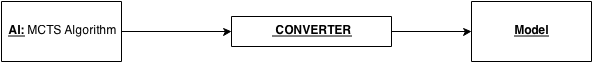
\includegraphics[width=0.80\textwidth]{2General_Architecture/2.2API/img/CONVERTER.png}
	\caption{Block Diagram of Converter}
	\label{fig:flowchart}
\end{figure}



The output of AI will be utilised by the Model in order to make a move on the board. It is possible that the output generated by the AI would be in the format that is not understandable by the Model. So there is a converter required to solve the purpose.

The converter will receive input from the MCTS algorithm module in some format such as tree. Then, it converts it into some other format that could be understood by the model such as a string or a binary code.

